\documentclass[12pt,a4paper]{report}

% ============ PACKAGES ============
\usepackage[utf8]{inputenc}
\usepackage[T1]{fontenc}
\usepackage[english]{babel}
\usepackage{geometry}
\usepackage{graphicx}
\usepackage{float}
\usepackage{booktabs}
\usepackage{array}
\usepackage{longtable}
\usepackage{xcolor}
\usepackage{listings}
\usepackage{fancyhdr}
\usepackage{titlesec}
\usepackage{hyperref}
\usepackage{tikz}
\usepackage{tikz-uml}
\usepackage{pgf-umlsd}
\usepackage{amsmath}
\usepackage{enumitem}
\usepackage{tocloft}
\usepackage{caption}
\usepackage{subcaption}

% ============ PAGE SETUP ============
\geometry{
    left=2.5cm,
    right=2.5cm,
    top=2.5cm,
    bottom=2.5cm
}

% ============ COLORS ============
\definecolor{codegreen}{rgb}{0,0.6,0}
\definecolor{codegray}{rgb}{0.5,0.5,0.5}
\definecolor{codepurple}{rgb}{0.58,0,0.82}
\definecolor{backcolour}{rgb}{0.95,0.95,0.92}
\definecolor{darkblue}{rgb}{0.0,0.0,0.6}
\definecolor{primarycolor}{RGB}{0,82,147}
\definecolor{secondarycolor}{RGB}{70,130,180}

% ============ CODE LISTING STYLE ============
\lstdefinestyle{javastyle}{
    backgroundcolor=\color{backcolour},
    commentstyle=\color{codegreen},
    keywordstyle=\color{darkblue}\bfseries,
    numberstyle=\tiny\color{codegray},
    stringstyle=\color{codepurple},
    basicstyle=\ttfamily\footnotesize,
    breakatwhitespace=false,
    breaklines=true,
    captionpos=b,
    keepspaces=true,
    numbers=left,
    numbersep=5pt,
    showspaces=false,
    showstringspaces=false,
    showtabs=false,
    tabsize=2,
    language=Java,
    frame=single,
    rulecolor=\color{black}
}

\lstset{style=javastyle}

% ============ HYPERREF SETUP ============
\hypersetup{
    colorlinks=true,
    linkcolor=primarycolor,
    filecolor=magenta,
    urlcolor=secondarycolor,
    pdftitle={Conservatoire Virtuel - Music School Management System},
    pdfauthor={Hassen Ben Amor, Dalil Adimi},
}

% ============ HEADER/FOOTER ============
\pagestyle{fancy}
\fancyhf{}
\fancyhead[L]{\leftmark}
\fancyhead[R]{Conservatoire Virtuel}
\fancyfoot[C]{\thepage}
\renewcommand{\headrulewidth}{0.4pt}
\renewcommand{\footrulewidth}{0.4pt}

% ============ CHAPTER FORMATTING ============
\titleformat{\chapter}[display]
{\normalfont\huge\bfseries\color{primarycolor}}
{\chaptertitlename\ \thechapter}{20pt}{\Huge}

\titleformat{\section}
{\normalfont\Large\bfseries\color{primarycolor}}
{\thesection}{1em}{}

\titleformat{\subsection}
{\normalfont\large\bfseries\color{secondarycolor}}
{\thesubsection}{1em}{}

% ============ DOCUMENT START ============
\begin{document}

% ============ TITLE PAGE ============
\begin{titlepage}
    \centering
    \vspace*{1cm}
    
    \includegraphics[width=0.3\textwidth]{university_logo.png}\\[1cm]
    % Note: Replace with your university logo or remove this line
    
    \textsc{\LARGE University Name}\\[0.5cm]
    \textsc{\Large Department of Computer Science}\\[1.5cm]
    
    \rule{\linewidth}{0.5mm}\\[0.4cm]
    {\huge\bfseries\color{primarycolor} Conservatoire Virtuel}\\[0.2cm]
    {\Large Music School Management System}\\[0.2cm]
    \rule{\linewidth}{0.5mm}\\[1.5cm]
    
    \Large\textbf{Object-Oriented Programming Project}\\[2cm]
    
    \begin{minipage}{0.4\textwidth}
        \begin{flushleft}
            \large\textbf{Authors:}\\
            Hassen \textsc{Ben Amor}\\
            Dalil \textsc{Adimi}
        \end{flushleft}
    \end{minipage}
    \begin{minipage}{0.4\textwidth}
        \begin{flushright}
            \large\textbf{Supervisor:}\\
            Prof. [Supervisor Name]\\[0.5cm]
            \textbf{Academic Year:}\\
            2024 -- 2025
        \end{flushright}
    \end{minipage}\\[2cm]
    
    \vfill
    {\large \today}
    
\end{titlepage}

% ============ ABSTRACT ============
\chapter*{Abstract}
\addcontentsline{toc}{chapter}{Abstract}

The \textbf{Conservatoire Virtuel} project is a comprehensive music school management system developed in Java. This application addresses the operational needs of a private music school, providing functionality for managing students, teachers, course packages, lesson scheduling, payments, and official examinations.

The system was designed with a strong emphasis on object-oriented programming principles, featuring abstract classes, interfaces, polymorphism, and copy constructors. The architecture follows best practices in software design, including the separation of concerns, encapsulation, and proper use of design patterns.

Key features include a robust scheduling system with conflict prevention, a flexible billing system supporting various service types, and an exam management module with capacity control and result tracking. The application demonstrates professional software development practices suitable for real-world deployment.

\textbf{Keywords:} Java, OOP, Music School, Management System, Scheduling, Billing, Abstract Classes, Interfaces, Polymorphism

% ============ TABLE OF CONTENTS ============
\tableofcontents
\listoffigures
\listoftables

% ============ CHAPTER 1: INTRODUCTION ============
\chapter{Introduction}

\section{Project Context}

A private music school called \textbf{Conservatoire Virtuel} requires an information system to support its internal activities. The objective is to design and implement an application that manages all aspects of school operations efficiently and professionally.

\section{Project Objectives}

The main objectives of this project are to:

\begin{enumerate}[label=\arabic*.]
    \item Design a comprehensive domain model for a music school
    \item Implement advanced object-oriented programming concepts
    \item Develop a functional console-based application
    \item Demonstrate proper software engineering practices
    \item Create professional documentation including UML diagrams
\end{enumerate}

\section{Scope}

The system manages the following aspects:

\begin{itemize}
    \item \textbf{People Management:} Students and teachers with their attributes and relationships
    \item \textbf{Service Management:} Course packages, individual lessons, and instrument rentals
    \item \textbf{Scheduling:} Lesson scheduling with conflict prevention and resource booking
    \item \textbf{Financial Management:} Payments, invoicing, and billing
    \item \textbf{Examination Management:} Official exams, registration, and results
\end{itemize}

\section{Document Structure}

This report is organized as follows:

\begin{itemize}
    \item \textbf{Chapter 2:} Requirements Analysis
    \item \textbf{Chapter 3:} System Design with UML
    \item \textbf{Chapter 4:} Implementation Details
    \item \textbf{Chapter 5:} OOP Concepts Discussion
    \item \textbf{Chapter 6:} Testing and Results
    \item \textbf{Chapter 7:} Conclusion
\end{itemize}

% ============ CHAPTER 2: REQUIREMENTS ============
\chapter{Requirements Analysis}

\section{Functional Requirements}

\subsection{Student Management}

A student is identified by a unique ID with the following attributes:
\begin{itemize}
    \item Last name, first name
    \item Address, date of birth, phone, email
    \item Level (Beginner/Intermediate/Advanced)
    \item Preferred instruments
\end{itemize}

Students can enroll in:
\begin{itemize}
    \item Course Packages (N lessons with validity dates)
    \item Individual lessons (billed per lesson)
\end{itemize}

The system tracks:
\begin{itemize}
    \item Purchased hours
    \item Remaining hours
    \item Usage history
\end{itemize}

\subsection{Teacher Management}

Each teacher has:
\begin{itemize}
    \item ID, name, qualifications
    \item Specializations (instruments they can teach)
    \item Hourly rate
    \item Availability schedule
\end{itemize}

\subsection{Course Packages and Services}

The school offers:
\begin{itemize}
    \item Music packages (fixed hours)
    \item Unlimited lessons packages
    \item Group or individual lessons
    \item Single paid lessons
    \item Instrument rental
    \item Room booking
\end{itemize}

\subsection{Scheduling System}

The system allows scheduling of:
\begin{itemize}
    \item Lessons (teacher + student + room + instrument)
    \item Room rentals
    \item Exam sessions
\end{itemize}

For each scheduled activity:
\begin{itemize}
    \item Date and start time
    \item Duration
    \item Assigned resources
    \item Status (scheduled/completed/cancelled)
\end{itemize}

\textbf{Important:} Schedule conflicts must be prevented.

\subsection{Exam Management}

The school organizes official exams:
\begin{itemize}
    \item Exams have a name, instrument, date, and capacity
    \item Students can register
    \item Results are recorded: pass/fail and optional score
\end{itemize}

\subsection{Payments and Billing}

The system tracks:
\begin{itemize}
    \item Payments
    \item Outstanding balances
    \item Prices of packages, rentals, and lessons
\end{itemize}

\section{Business Rules}

\begin{enumerate}
    \item Package hours expire at the package end date
    \item If a lesson is cancelled less than 24 hours before, it counts as consumed
    \item Exam registration closes when maximum capacity is reached
    \item A group lesson consumes one hour from each participant
\end{enumerate}

\section{Non-Functional Requirements}

\begin{itemize}
    \item \textbf{Maintainability:} Clean, well-documented code
    \item \textbf{Extensibility:} Easy to add new features
    \item \textbf{Reliability:} Proper error handling
    \item \textbf{Usability:} Intuitive console interface
\end{itemize}

% ============ CHAPTER 3: SYSTEM DESIGN ============
\chapter{System Design}

\section{Architecture Overview}

The system follows a layered architecture:

\begin{enumerate}
    \item \textbf{Presentation Layer:} Console-based user interface (\texttt{ConservatoireApp})
    \item \textbf{Service Layer:} Business logic (\texttt{SchedulingService}, \texttt{PaymentService}, \texttt{ExamService})
    \item \textbf{Repository Layer:} Data storage (\texttt{DataRepository})
    \item \textbf{Model Layer:} Domain entities (Person, Service, ScheduledActivity, etc.)
\end{enumerate}

\section{Package Structure}

\begin{figure}[H]
\centering
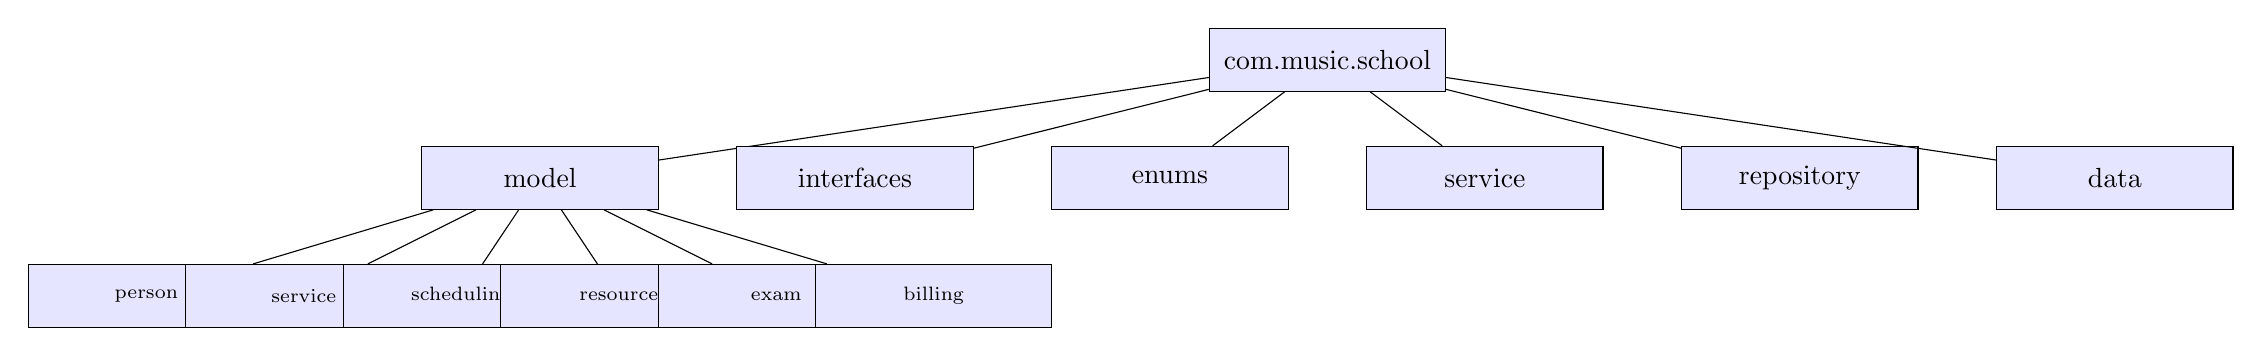
\begin{tikzpicture}[
    package/.style={draw, rectangle, minimum width=3cm, minimum height=0.8cm, fill=blue!10},
    level 1/.style={sibling distance=4cm},
    level 2/.style={sibling distance=2cm}
]
\node[package] {com.music.school}
    child {node[package] {model}
        child {node[package, font=\scriptsize] {person}}
        child {node[package, font=\scriptsize] {service}}
        child {node[package, font=\scriptsize] {scheduling}}
        child {node[package, font=\scriptsize] {resource}}
        child {node[package, font=\scriptsize] {exam}}
        child {node[package, font=\scriptsize] {billing}}
    }
    child {node[package] {interfaces}}
    child {node[package] {enums}}
    child {node[package] {service}}
    child {node[package] {repository}}
    child {node[package] {data}};
\end{tikzpicture}
\caption{Package Structure Diagram}
\label{fig:packages}
\end{figure}

\section{Class Diagram}

\subsection{Person Hierarchy}

\begin{figure}[H]
\centering
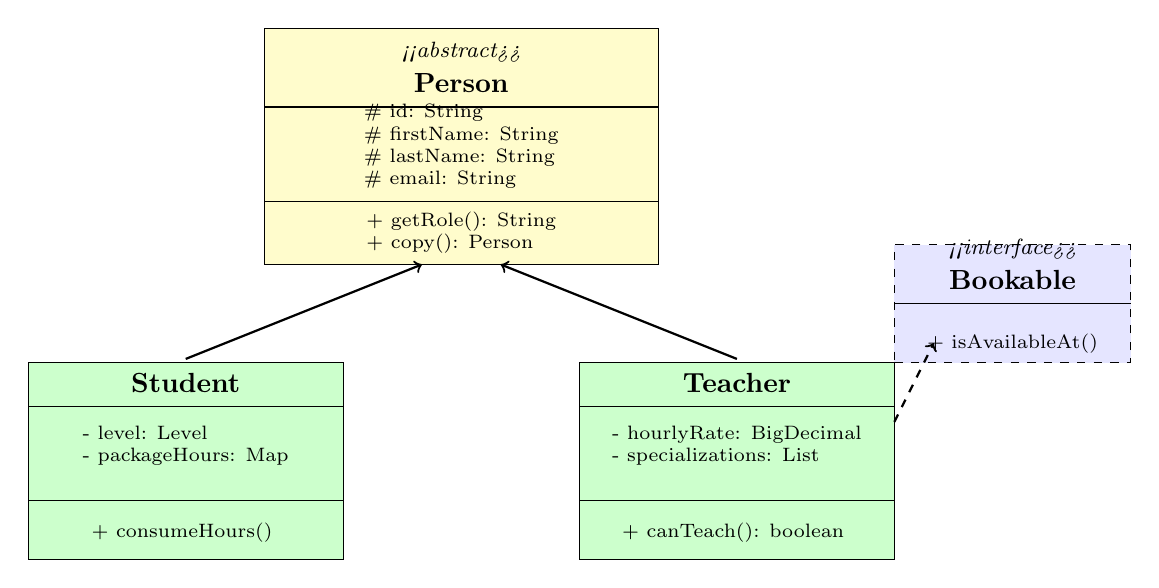
\begin{tikzpicture}
    % Abstract Person class
    \node[draw, rectangle, minimum width=5cm, minimum height=3cm, fill=yellow!20] (person) at (0,0) {};
    \node[font=\footnotesize\itshape] at (0, 1.2) {<<abstract>>};
    \node[font=\bfseries] at (0, 0.8) {Person};
    \draw (-2.5, 0.5) -- (2.5, 0.5);
    \node[font=\scriptsize, align=left] at (0, 0) {
        \# id: String\\
        \# firstName: String\\
        \# lastName: String\\
        \# email: String
    };
    \draw (-2.5, -0.7) -- (2.5, -0.7);
    \node[font=\scriptsize, align=left] at (0, -1.1) {
        + getRole(): String\\
        + copy(): Person
    };
    
    % Student class
    \node[draw, rectangle, minimum width=4cm, minimum height=2.5cm, fill=green!20] (student) at (-3.5,-4) {};
    \node[font=\bfseries] at (-3.5, -3) {Student};
    \draw (-5.5, -3.3) -- (-1.5, -3.3);
    \node[font=\scriptsize, align=left] at (-3.5, -3.8) {
        - level: Level\\
        - packageHours: Map
    };
    \draw (-5.5, -4.5) -- (-1.5, -4.5);
    \node[font=\scriptsize, align=left] at (-3.5, -4.9) {
        + consumeHours()
    };
    
    % Teacher class
    \node[draw, rectangle, minimum width=4cm, minimum height=2.5cm, fill=green!20] (teacher) at (3.5,-4) {};
    \node[font=\bfseries] at (3.5, -3) {Teacher};
    \draw (1.5, -3.3) -- (5.5, -3.3);
    \node[font=\scriptsize, align=left] at (3.5, -3.8) {
        - hourlyRate: BigDecimal\\
        - specializations: List
    };
    \draw (1.5, -4.5) -- (5.5, -4.5);
    \node[font=\scriptsize, align=left] at (3.5, -4.9) {
        + canTeach(): boolean
    };
    
    % Inheritance arrows
    \draw[->, thick] (-3.5, -2.7) -- (-0.5, -1.5);
    \draw[->, thick] (3.5, -2.7) -- (0.5, -1.5);
    
    % Bookable interface
    \node[draw, rectangle, dashed, minimum width=3cm, minimum height=1.5cm, fill=blue!10] (bookable) at (7,-2) {};
    \node[font=\footnotesize\itshape] at (7, -1.3) {<<interface>>};
    \node[font=\bfseries] at (7, -1.7) {Bookable};
    \draw (5.5, -2) -- (8.5, -2);
    \node[font=\scriptsize] at (7, -2.5) {+ isAvailableAt()};
    
    % Implementation arrow
    \draw[->, dashed, thick] (5.5, -3.5) -- (6, -2.5);
    
\end{tikzpicture}
\caption{Person Class Hierarchy}
\label{fig:person-hierarchy}
\end{figure}

\subsection{Service Hierarchy}

\begin{figure}[H]
\centering
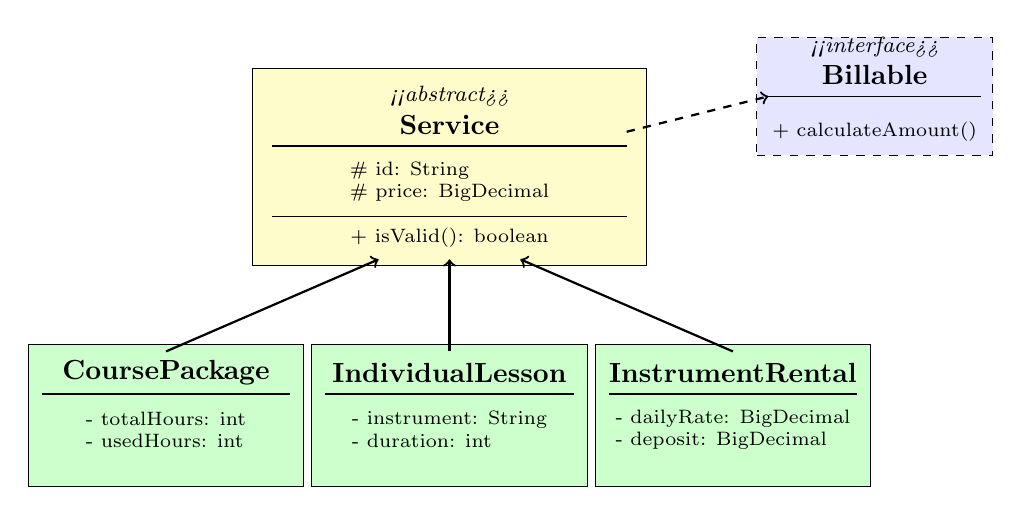
\begin{tikzpicture}[scale=0.9]
    % Billable interface
    \node[draw, rectangle, dashed, minimum width=3cm, minimum height=1.5cm, fill=blue!10] (billable) at (6,1) {};
    \node[font=\footnotesize\itshape] at (6, 1.7) {<<interface>>};
    \node[font=\bfseries] at (6, 1.3) {Billable};
    \draw (4.5, 1) -- (7.5, 1);
    \node[font=\scriptsize] at (6, 0.5) {+ calculateAmount()};
    
    % Abstract Service class
    \node[draw, rectangle, minimum width=5cm, minimum height=2.5cm, fill=yellow!20] (service) at (0,0) {};
    \node[font=\footnotesize\itshape] at (0, 1) {<<abstract>>};
    \node[font=\bfseries] at (0, 0.6) {Service};
    \draw (-2.5, 0.3) -- (2.5, 0.3);
    \node[font=\scriptsize, align=left] at (0, -0.2) {
        \# id: String\\
        \# price: BigDecimal
    };
    \draw (-2.5, -0.7) -- (2.5, -0.7);
    \node[font=\scriptsize] at (0, -1) {+ isValid(): boolean};
    
    % Implementation arrow
    \draw[->, dashed, thick] (2.5, 0.5) -- (4.5, 1);
    
    % CoursePackage
    \node[draw, rectangle, minimum width=3.5cm, minimum height=1.8cm, fill=green!20] (pkg) at (-4,-3.5) {};
    \node[font=\bfseries] at (-4, -2.9) {CoursePackage};
    \draw (-5.75, -3.2) -- (-2.25, -3.2);
    \node[font=\scriptsize, align=left] at (-4, -3.7) {
        - totalHours: int\\
        - usedHours: int
    };
    
    % IndividualLesson
    \node[draw, rectangle, minimum width=3.5cm, minimum height=1.8cm, fill=green!20] (ind) at (0,-3.5) {};
    \node[font=\bfseries] at (0, -2.9) {IndividualLesson};
    \draw (-1.75, -3.2) -- (1.75, -3.2);
    \node[font=\scriptsize, align=left] at (0, -3.7) {
        - instrument: String\\
        - duration: int
    };
    
    % InstrumentRental
    \node[draw, rectangle, minimum width=3.5cm, minimum height=1.8cm, fill=green!20] (rental) at (4,-3.5) {};
    \node[font=\bfseries] at (4, -2.9) {InstrumentRental};
    \draw (2.25, -3.2) -- (5.75, -3.2);
    \node[font=\scriptsize, align=left] at (4, -3.7) {
        - dailyRate: BigDecimal\\
        - deposit: BigDecimal
    };
    
    % Inheritance arrows
    \draw[->, thick] (-4, -2.6) -- (-1, -1.3);
    \draw[->, thick] (0, -2.6) -- (0, -1.3);
    \draw[->, thick] (4, -2.6) -- (1, -1.3);
    
\end{tikzpicture}
\caption{Service Class Hierarchy}
\label{fig:service-hierarchy}
\end{figure}

\subsection{Complete Class Diagram}

\begin{table}[H]
\centering
\caption{Summary of Classes and Their Relationships}
\label{tab:classes}
\begin{tabular}{|l|l|l|p{5cm}|}
\hline
\textbf{Class} & \textbf{Type} & \textbf{Parent/Interface} & \textbf{Description} \\
\hline
Person & Abstract & - & Base class for all people \\
Student & Concrete & Person & Music school student \\
Teacher & Concrete & Person, Bookable & Music teacher \\
\hline
Service & Abstract & Billable & Base for all services \\
CoursePackage & Concrete & Service & Package of lessons \\
IndividualLesson & Concrete & Service & Single lesson service \\
InstrumentRental & Concrete & Service & Instrument rental \\
\hline
ScheduledActivity & Abstract & Schedulable & Base for scheduled items \\
Lesson & Concrete & ScheduledActivity & Scheduled lesson \\
RoomBooking & Concrete & ScheduledActivity & Room reservation \\
\hline
Room & Concrete & Bookable & Practice/lesson room \\
Instrument & Concrete & Bookable & Musical instrument \\
Exam & Concrete & - & Official examination \\
Invoice & Concrete & - & Billing invoice \\
Payment & Concrete & - & Payment record \\
\hline
\end{tabular}
\end{table}

\section{Sequence Diagram: Scheduling a Lesson}

The following sequence diagram illustrates the process of scheduling a new lesson:

\begin{figure}[H]
\centering
\begin{tikzpicture}[scale=0.7]
    % Actors/Objects
    \node[draw, rectangle, fill=blue!20, minimum width=2cm] (user) at (0,0) {User};
    \node[draw, rectangle, fill=green!20, minimum width=2cm] (sched) at (4,0) {SchedulingService};
    \node[draw, rectangle, fill=yellow!20, minimum width=2cm] (repo) at (8,0) {DataRepository};
    \node[draw, rectangle, fill=orange!20, minimum width=2cm] (teacher) at (12,0) {Teacher};
    \node[draw, rectangle, fill=purple!20, minimum width=2cm] (room) at (16,0) {Room};
    
    % Lifelines
    \draw[dashed] (0,-0.5) -- (0,-14);
    \draw[dashed] (4,-0.5) -- (4,-14);
    \draw[dashed] (8,-0.5) -- (8,-14);
    \draw[dashed] (12,-0.5) -- (12,-14);
    \draw[dashed] (16,-0.5) -- (16,-14);
    
    % Messages
    \draw[->, thick] (0,-1) -- (4,-1) node[midway, above, font=\scriptsize] {1: scheduleLesson()};
    \draw[->, thick] (4,-2) -- (8,-2) node[midway, above, font=\scriptsize] {2: getTeacher(id)};
    \draw[<--, thick] (4,-2.5) -- (8,-2.5) node[midway, above, font=\scriptsize] {teacher};
    
    \draw[->, thick] (4,-3.5) -- (12,-3.5) node[midway, above, font=\scriptsize] {3: canTeach(instrument)};
    \draw[<--, thick] (4,-4) -- (12,-4) node[midway, above, font=\scriptsize] {true};
    
    \draw[->, thick] (4,-5) -- (8,-5) node[midway, above, font=\scriptsize] {4: checkConflicts()};
    \draw[<--, thick] (4,-5.5) -- (8,-5.5) node[midway, above, font=\scriptsize] {no conflicts};
    
    \draw[->, thick] (4,-6.5) -- (12,-6.5) node[midway, above, font=\scriptsize] {5: isAvailableAt()};
    \draw[<--, thick] (4,-7) -- (12,-7) node[midway, above, font=\scriptsize] {true};
    
    \draw[->, thick] (4,-8) -- (16,-8) node[midway, above, font=\scriptsize] {6: isAvailableAt()};
    \draw[<--, thick] (4,-8.5) -- (16,-8.5) node[midway, above, font=\scriptsize] {true};
    
    \draw[->, thick] (4,-9.5) -- (12,-9.5) node[midway, above, font=\scriptsize] {7: addBooking()};
    \draw[->, thick] (4,-10.5) -- (16,-10.5) node[midway, above, font=\scriptsize] {8: addBooking()};
    
    \draw[->, thick] (4,-11.5) -- (8,-11.5) node[midway, above, font=\scriptsize] {9: addScheduledActivity()};
    
    \draw[<--, thick] (0,-13) -- (4,-13) node[midway, above, font=\scriptsize] {10: return Lesson};
    
\end{tikzpicture}
\caption{Sequence Diagram: Lesson Scheduling}
\label{fig:sequence-scheduling}
\end{figure}

\section{Activity Diagram: Exam Registration}

\begin{figure}[H]
\centering
\begin{tikzpicture}[
    node distance=1.2cm,
    start/.style={circle, draw, fill=black, minimum size=0.5cm},
    end/.style={circle, draw, fill=black, minimum size=0.5cm, double},
    activity/.style={rectangle, draw, rounded corners, fill=blue!20, minimum width=3cm, minimum height=0.8cm},
    decision/.style={diamond, draw, fill=yellow!20, aspect=2, minimum width=2cm},
    arrow/.style={->, thick}
]
    % Start
    \node[start] (start) {};
    
    % Activities
    \node[activity, below=of start] (select) {Select Exam};
    \node[decision, below=of select] (open) {Registration Open?};
    \node[decision, below=of open] (deadline) {Before Deadline?};
    \node[decision, below=of deadline] (capacity) {Spots Available?};
    \node[decision, below=of capacity] (registered) {Already Registered?};
    \node[activity, below=of registered] (create) {Create Registration};
    \node[activity, below=of create] (success) {Return Success};
    
    % Error node
    \node[activity, right=3cm of deadline, fill=red!20] (error) {Return Error};
    
    % End
    \node[end, below=of success] (end) {};
    
    % Arrows
    \draw[arrow] (start) -- (select);
    \draw[arrow] (select) -- (open);
    \draw[arrow] (open) -- node[left] {Yes} (deadline);
    \draw[arrow] (deadline) -- node[left] {Yes} (capacity);
    \draw[arrow] (capacity) -- node[left] {Yes} (registered);
    \draw[arrow] (registered) -- node[left] {No} (create);
    \draw[arrow] (create) -- (success);
    \draw[arrow] (success) -- (end);
    
    % Error paths
    \draw[arrow] (open.east) -- node[above] {No} (error.west);
    \draw[arrow] (deadline.east) -- node[above] {No} (error);
    \draw[arrow] (capacity.east) -| node[above, pos=0.3] {No} (error);
    \draw[arrow] (registered.east) -| node[above, pos=0.3] {Yes} (error);
    \draw[arrow] (error) |- (end);
    
\end{tikzpicture}
\caption{Activity Diagram: Exam Registration Process}
\label{fig:activity-exam}
\end{figure}

% ============ CHAPTER 4: IMPLEMENTATION ============
\chapter{Implementation Details}

\section{Technology Stack}

\begin{itemize}
    \item \textbf{Language:} Java 17
    \item \textbf{Build Tool:} Maven 3.x
    \item \textbf{IDE:} IntelliJ IDEA / VS Code
\end{itemize}

\section{Project Structure}

\begin{lstlisting}[language=bash, caption={Project Directory Structure}]
java-project/
├── pom.xml
├── README.md
└── src/main/java/com/music/school/
    ├── ConservatoireApp.java
    ├── enums/
    │   ├── Level.java
    │   ├── ActivityStatus.java
    │   ├── PaymentStatus.java
    │   ├── ServiceType.java
    │   └── ExamResult.java
    ├── interfaces/
    │   ├── Schedulable.java
    │   ├── Billable.java
    │   └── Bookable.java
    ├── model/
    │   ├── person/
    │   ├── service/
    │   ├── scheduling/
    │   ├── resource/
    │   ├── exam/
    │   └── billing/
    ├── service/
    ├── repository/
    └── data/
\end{lstlisting}

\section{Key Implementation Details}

\subsection{Abstract Person Class}

\begin{lstlisting}[caption={Person Abstract Class}]
public abstract class Person {
    protected String id;
    protected String firstName;
    protected String lastName;
    protected String email;
    protected LocalDate dateOfBirth;
    
    // Copy constructor
    protected Person(Person other) {
        this.id = other.id;
        this.firstName = other.firstName;
        this.lastName = other.lastName;
        this.email = other.email;
        this.dateOfBirth = other.dateOfBirth;
    }
    
    // Abstract methods
    protected abstract String getIdPrefix();
    public abstract String getRole();
    public abstract Person copy();
    
    public String getFullName() {
        return firstName + " " + lastName;
    }
}
\end{lstlisting}

\subsection{Schedulable Interface}

\begin{lstlisting}[caption={Schedulable Interface with Default Methods}]
public interface Schedulable {
    LocalDateTime getScheduledDateTime();
    Duration getDuration();
    ActivityStatus getStatus();
    
    default LocalDateTime getEndDateTime() {
        return getScheduledDateTime().plus(getDuration());
    }
    
    default boolean conflictsWith(Schedulable other) {
        LocalDateTime thisStart = this.getScheduledDateTime();
        LocalDateTime thisEnd = this.getEndDateTime();
        LocalDateTime otherStart = other.getScheduledDateTime();
        LocalDateTime otherEnd = other.getEndDateTime();
        
        return thisStart.isBefore(otherEnd) && 
               thisEnd.isAfter(otherStart);
    }
    
    default boolean canCancelWithoutPenalty() {
        return LocalDateTime.now().plusHours(24)
            .isBefore(getScheduledDateTime());
    }
}
\end{lstlisting}

\subsection{Conflict Detection in Scheduling}

\begin{lstlisting}[caption={Scheduling Conflict Detection}]
public List<String> checkSchedulingConflicts(
        String teacherId, List<String> studentIds,
        String roomId, LocalDateTime dateTime, 
        int durationMinutes) {
    
    List<String> conflicts = new ArrayList<>();
    
    // Check teacher conflicts
    List<Lesson> teacherLessons = repository
        .getTeacherLessons(teacherId);
    for (Lesson lesson : teacherLessons) {
        if (lesson.getStatus() == ActivityStatus.SCHEDULED 
            && tempSchedulable.conflictsWith(lesson)) {
            conflicts.add("Teacher has another lesson");
        }
    }
    
    // Check room conflicts
    List<ScheduledActivity> roomActivities = repository
        .getRoomActivities(roomId);
    for (ScheduledActivity activity : roomActivities) {
        if (tempSchedulable.conflictsWith(activity)) {
            conflicts.add("Room is already booked");
        }
    }
    
    return conflicts;
}
\end{lstlisting}

\subsection{Polymorphic Billing}

\begin{lstlisting}[caption={Polymorphic Use of Billable Interface}]
public void addBillableToInvoice(String invoiceId, 
        Billable billable) {
    Invoice invoice = repository.getInvoice(invoiceId);
    
    // Polymorphic call - works for any Billable
    InvoiceItem item = new InvoiceItem(
        billable.getBillingId(),
        billable.getBillingDescription(),
        1,
        billable.calculateAmount()  // Polymorphic method
    );
    
    invoice.addItem(item);
}

// Usage with different service types:
List<Billable> billables = new ArrayList<>();
billables.addAll(packages);     // CoursePackage
billables.addAll(lessons);      // IndividualLesson
billables.addAll(rentals);      // InstrumentRental

for (Billable b : billables) {
    paymentService.addBillableToInvoice(invoiceId, b);
}
\end{lstlisting}

% ============ CHAPTER 5: OOP CONCEPTS ============
\chapter{Object-Oriented Programming Concepts}

\section{Abstract Classes}

The system implements three abstract classes:

\subsection{Person (Abstract)}

\begin{itemize}
    \item \textbf{Purpose:} Generalization of common attributes for students and teachers
    \item \textbf{Extended by:} \texttt{Student}, \texttt{Teacher}
    \item \textbf{Abstract methods:} \texttt{getIdPrefix()}, \texttt{getRole()}, \texttt{copy()}
\end{itemize}

\subsection{Service (Abstract)}

\begin{itemize}
    \item \textbf{Purpose:} Base class for all billable services
    \item \textbf{Extended by:} \texttt{CoursePackage}, \texttt{IndividualLesson}, \texttt{InstrumentRental}
    \item \textbf{Implements:} \texttt{Billable} interface
    \item \textbf{Abstract methods:} \texttt{getIdPrefix()}, \texttt{isValid()}, \texttt{copy()}
\end{itemize}

\subsection{ScheduledActivity (Abstract)}

\begin{itemize}
    \item \textbf{Purpose:} Base class for all scheduled activities
    \item \textbf{Extended by:} \texttt{Lesson}, \texttt{RoomBooking}
    \item \textbf{Implements:} \texttt{Schedulable} interface
    \item \textbf{Abstract methods:} \texttt{getActivityType()}, \texttt{consumesLessonHours()}
\end{itemize}

\section{Interfaces}

The system defines three interfaces:

\subsection{Schedulable Interface}

\begin{table}[H]
\centering
\caption{Schedulable Interface Methods}
\begin{tabular}{|l|l|}
\hline
\textbf{Method} & \textbf{Description} \\
\hline
\texttt{getScheduledDateTime()} & Get scheduled date/time \\
\texttt{getDuration()} & Get activity duration \\
\texttt{getStatus()} & Get current status \\
\texttt{conflictsWith()} & Check time overlap (default) \\
\texttt{canCancelWithoutPenalty()} & 24h check (default) \\
\hline
\end{tabular}
\end{table}

\subsection{Billable Interface}

\begin{table}[H]
\centering
\caption{Billable Interface Methods}
\begin{tabular}{|l|l|}
\hline
\textbf{Method} & \textbf{Description} \\
\hline
\texttt{getBillingId()} & Get unique billing ID \\
\texttt{getServiceType()} & Get service type \\
\texttt{calculateAmount()} & Calculate total amount \\
\texttt{getBillingDescription()} & Get description for invoice \\
\texttt{isPaid()} & Check payment status \\
\texttt{markAsPaid()} & Mark as paid \\
\hline
\end{tabular}
\end{table}

\subsection{Bookable Interface}

\begin{table}[H]
\centering
\caption{Bookable Interface Methods}
\begin{tabular}{|l|l|}
\hline
\textbf{Method} & \textbf{Description} \\
\hline
\texttt{getResourceId()} & Get resource identifier \\
\texttt{isAvailableAt()} & Check availability \\
\texttt{getBookedSlots()} & Get all bookings \\
\texttt{addBooking()} & Add new booking \\
\texttt{removeBooking()} & Cancel booking \\
\hline
\end{tabular}
\end{table}

\section{Polymorphism}

\subsection{Polymorphic Collections}

\begin{lstlisting}[caption={Polymorphic Collections Example}]
// List of Person containing both Student and Teacher
List<Person> people = new ArrayList<>();
people.addAll(repository.getAllStudents());
people.addAll(repository.getAllTeachers());

for (Person person : people) {
    // Dynamic dispatch - different output for each type
    System.out.println(person.getRole());
    System.out.println(person.getDetailedInfo());
}
\end{lstlisting}

\subsection{Polymorphic Method Calls}

\begin{lstlisting}[caption={Polymorphic Method Calls}]
// Service hierarchy - all implement Billable
List<Service> services = repository.getAllServices();

BigDecimal totalRevenue = BigDecimal.ZERO;
for (Service service : services) {
    // calculateAmount() implemented differently
    // in CoursePackage, IndividualLesson, InstrumentRental
    totalRevenue = totalRevenue.add(service.calculateAmount());
}
\end{lstlisting}

\subsection{Dynamic Dispatch}

The system demonstrates dynamic dispatch through:
\begin{itemize}
    \item \texttt{getRole()} returns "Student" or "Teacher"
    \item \texttt{getActivityType()} returns "Individual Lesson" or "Room Booking"
    \item \texttt{calculateAmount()} computes differently for each service type
    \item \texttt{isValid()} has different logic per service type
\end{itemize}

\section{Copy Constructors}

Copy constructors are implemented in all major classes to support deep copying:

\begin{lstlisting}[caption={Copy Constructor Implementation}]
public class Student extends Person {
    private Level level;
    private List<String> preferredInstruments;
    private Map<String, Integer> packageHours;
    
    // Copy constructor
    public Student(Student other) {
        super(other);  // Call parent copy constructor
        this.level = other.level;
        // Deep copy of collections
        this.preferredInstruments = 
            new ArrayList<>(other.preferredInstruments);
        this.packageHours = 
            new HashMap<>(other.packageHours);
    }
    
    @Override
    public Person copy() {
        return new Student(this);
    }
}
\end{lstlisting}

\textbf{Classes with copy constructors:}
\begin{itemize}
    \item \texttt{Student}, \texttt{Teacher}
    \item \texttt{CoursePackage}, \texttt{IndividualLesson}, \texttt{InstrumentRental}
    \item \texttt{Lesson}, \texttt{RoomBooking}
    \item \texttt{Room}, \texttt{Instrument}
    \item \texttt{Exam}, \texttt{Invoice}, \texttt{Payment}
\end{itemize}

\section{Encapsulation}

The system demonstrates proper encapsulation through:

\subsection{Private Fields}
All class fields are declared as \texttt{private} or \texttt{protected}.

\subsection{Defensive Copies}
Getters return defensive copies of mutable collections:

\begin{lstlisting}[caption={Defensive Copy in Getter}]
public List<String> getPreferredInstruments() {
    // Return a new list to protect internal state
    return new ArrayList<>(preferredInstruments);
}

public Map<String, Integer> getPackageHours() {
    // Return a new map to prevent external modification
    return new HashMap<>(packageHours);
}
\end{lstlisting}

\subsection{Validation in Setters}
Setters validate input data before assignment.

\section{Composition vs Inheritance}

\begin{table}[H]
\centering
\caption{Composition and Inheritance Usage}
\begin{tabular}{|l|l|l|}
\hline
\textbf{Relationship} & \textbf{Type} & \textbf{Example} \\
\hline
Student extends Person & Inheritance & IS-A relationship \\
Teacher extends Person & Inheritance & IS-A relationship \\
CoursePackage extends Service & Inheritance & IS-A relationship \\
\hline
Teacher HAS TimeRanges & Composition & HAS-A relationship \\
Exam HAS ExamRegistrations & Composition & HAS-A relationship \\
Invoice HAS InvoiceItems & Composition & HAS-A relationship \\
\hline
\end{tabular}
\end{table}

% ============ CHAPTER 6: TESTING ============
\chapter{Testing and Results}

\section{Test Data Scenario}

The system is initialized with comprehensive test data:

\subsection{People}
\begin{itemize}
    \item \textbf{8 Students:} Including 3 minors with guardian information
    \item \textbf{5 Teachers:} Piano, Violin, Guitar, Drums, Flute specialists
\end{itemize}

\subsection{Resources}
\begin{itemize}
    \item \textbf{8 Rooms:} Piano Studios, String Room, Guitar Studio, Percussion Room, Ensemble Hall, Practice Rooms
    \item \textbf{7 Instruments:} Violins, Guitars, Cello, Flute, Clarinet
\end{itemize}

\subsection{Services}
\begin{itemize}
    \item 5 Course Packages (standard and unlimited)
    \item 1 Individual Lesson
    \item 1 Instrument Rental
\end{itemize}

\subsection{Scheduled Activities}
\begin{itemize}
    \item Multiple lessons for the coming week
    \item Group lesson example
\end{itemize}

\subsection{Exams}
\begin{itemize}
    \item 4 upcoming exams (Piano, Violin, Guitar, Music Theory)
    \item 1 past exam with recorded results
\end{itemize}

\section{Screenshots of Execution}

\subsection{Main Menu}

\begin{verbatim}
╔══════════════════════════════════════════╗
║              MAIN MENU                   ║
╠══════════════════════════════════════════╣
║  1. Manage Students and Teachers         ║
║  2. Manage Course Packages & Lessons     ║
║  3. Manage Scheduling and Booking        ║
║  4. Manage Payments and Billing          ║
║  5. Manage Exams and Results             ║
║  6. Demonstrate OOP Concepts             ║
║  0. Exit                                 ║
╚══════════════════════════════════════════╝
\end{verbatim}

\subsection{Student Listing}

\begin{verbatim}
═══ ALL STUDENTS (8) ═══
ID              Name                      Level           Hours Left   Instruments
────────────────────────────────────────────────────────────────────────────────────
STU-A1B2C3D4    Alice Moreau              Intermediate    8            Piano
STU-E5F6G7H8    Thomas Leroy              Beginner        6            Guitar, Bass
STU-I9J0K1L2    Emma Dubois               Advanced        Unlimited    Violin
...
\end{verbatim}

\subsection{Scheduling a Lesson}

\begin{verbatim}
═══ SCHEDULE NEW LESSON ═══

Enter teacher ID: TCH-M1N2O3P4
Enter student ID(s): STU-A1B2C3D4
Enter room ID: ROOM-Q5R6S7
Instrument: Piano
Date and time (yyyy-MM-dd HH:mm): 2025-01-15 10:00
Duration (minutes): 60

✓ Lesson scheduled successfully!
═══════════════════════════════════════
           LESSON INFORMATION          
═══════════════════════════════════════
ID:          LES-T8U9V0W1
Type:        Individual Lesson
Instrument:  Piano
Date/Time:   2025-01-15T10:00
Duration:    60 minutes
Teacher ID:  TCH-M1N2O3P4
Students:    STU-A1B2C3D4
Status:      Scheduled
═══════════════════════════════════════
\end{verbatim}

\subsection{OOP Demonstrations}

\begin{verbatim}
════════════════════════════════════════════════════════════════
        OBJECT-ORIENTED PROGRAMMING DEMONSTRATIONS
════════════════════════════════════════════════════════════════

1. ABSTRACT CLASSES
────────────────────────────────────────
The system uses two main abstract classes:
  • Person - Base class for Student and Teacher
  • Service - Base class for CoursePackage, IndividualLesson
  • ScheduledActivity - Base class for Lesson, RoomBooking

Polymorphic Person collection:
  Total people in system: 13
    Alice Moreau - Role: Student
    Thomas Leroy - Role: Student
    Marie Dupont - Role: Teacher

2. INTERFACES
────────────────────────────────────────
  • Schedulable - For lessons, room bookings
  • Billable - For services that can be invoiced
  • Bookable - For resources (rooms, instruments, teachers)
\end{verbatim}

\section{Business Rule Verification}

\subsection{24-Hour Cancellation Policy}

\begin{verbatim}
Enter activity ID to cancel: LES-X1Y2Z3A4

✓ Activity cancelled (within 24h - counts as consumed).
\end{verbatim}

\subsection{Exam Capacity Limit}

\begin{verbatim}
═══ REGISTER STUDENT FOR EXAM ═══

Enter exam ID: EXM-B5C6D7E8
Enter student ID: STU-F9G0H1I2

✗ Error: Exam is at maximum capacity
\end{verbatim}

\subsection{Scheduling Conflict Detection}

\begin{verbatim}
✗ Error: Scheduling conflicts detected:
  - Teacher has another lesson: LES-J3K4L5M6 at 2025-01-15T10:00
  - Room has another booking: BKG-N7O8P9Q0 at 2025-01-15T10:00
\end{verbatim}

% ============ CHAPTER 7: CONCLUSION ============
\chapter{Conclusion}

\section{Summary}

The \textbf{Conservatoire Virtuel} project successfully implements a comprehensive music school management system that meets all specified requirements. The application demonstrates:

\begin{itemize}
    \item Proper use of object-oriented programming principles
    \item Clean architecture with separation of concerns
    \item Robust business logic implementation
    \item User-friendly console interface
\end{itemize}

\section{OOP Requirements Fulfilled}

\begin{table}[H]
\centering
\caption{OOP Requirements Checklist}
\begin{tabular}{|l|c|l|}
\hline
\textbf{Requirement} & \textbf{Status} & \textbf{Implementation} \\
\hline
Abstract Classes (2+) & \checkmark & Person, Service, ScheduledActivity \\
Interfaces (2+) & \checkmark & Schedulable, Billable, Bookable \\
Polymorphism & \checkmark & Collections, method calls \\
Copy Constructors & \checkmark & All major classes \\
Inheritance & \checkmark & Multiple hierarchies \\
Composition & \checkmark & Teacher-TimeRange, Exam-Registration \\
Encapsulation & \checkmark & Private fields, defensive copies \\
\hline
\end{tabular}
\end{table}

\section{Lessons Learned}

Through this project, we gained valuable experience in:

\begin{enumerate}
    \item Designing object-oriented systems from requirements
    \item Implementing abstract classes and interfaces effectively
    \item Managing polymorphic collections and method calls
    \item Creating defensive copies to protect object state
    \item Developing clean, maintainable code
\end{enumerate}

\section{Future Improvements}

Potential enhancements for future versions:

\begin{itemize}
    \item Database integration (MySQL/PostgreSQL)
    \item Graphical user interface (JavaFX)
    \item REST API for web/mobile access
    \item Automated scheduling suggestions
    \item Email notifications
    \item Financial reporting with charts
    \item Multi-language support
\end{itemize}

\section{Acknowledgments}

We would like to thank our professor for the guidance and support throughout this project.

% ============ APPENDIX ============
\appendix

\chapter{Source Code Listings}

\section{Complete Interface Definitions}

\begin{lstlisting}[caption={Schedulable.java}]
package com.music.school.interfaces;

import com.music.school.enums.ActivityStatus;
import java.time.LocalDateTime;
import java.time.Duration;

public interface Schedulable {
    LocalDateTime getScheduledDateTime();
    void setScheduledDateTime(LocalDateTime dateTime);
    Duration getDuration();
    void setDuration(Duration duration);
    ActivityStatus getStatus();
    void setStatus(ActivityStatus status);
    
    default LocalDateTime getEndDateTime() {
        return getScheduledDateTime().plus(getDuration());
    }
    
    default boolean conflictsWith(Schedulable other) {
        if (other == null) return false;
        LocalDateTime thisStart = this.getScheduledDateTime();
        LocalDateTime thisEnd = this.getEndDateTime();
        LocalDateTime otherStart = other.getScheduledDateTime();
        LocalDateTime otherEnd = other.getEndDateTime();
        return thisStart.isBefore(otherEnd) && 
               thisEnd.isAfter(otherStart);
    }
    
    default boolean canCancelWithoutPenalty() {
        return LocalDateTime.now().plusHours(24)
            .isBefore(getScheduledDateTime());
    }
}
\end{lstlisting}

\chapter{How to Run}

\section{Prerequisites}
\begin{itemize}
    \item Java JDK 17 or higher
    \item Maven 3.6 or higher
\end{itemize}

\section{Build and Run Commands}

\begin{lstlisting}[language=bash]
# Navigate to project directory
cd java-project

# Compile the project
mvn clean compile

# Run the application
mvn exec:java -Dexec.mainClass="com.music.school.ConservatoireApp"

# Or package and run as JAR
mvn package
java -jar target/conservatoire-virtuel-1.0.0.jar
\end{lstlisting}

% ============ BIBLIOGRAPHY ============
\begin{thebibliography}{9}

\bibitem{java17}
Oracle Corporation,
\textit{Java SE 17 Documentation},
2021.
\url{https://docs.oracle.com/en/java/javase/17/}

\bibitem{oop}
Bertrand Meyer,
\textit{Object-Oriented Software Construction},
Prentice Hall, 2nd Edition, 1997.

\bibitem{cleancode}
Robert C. Martin,
\textit{Clean Code: A Handbook of Agile Software Craftsmanship},
Prentice Hall, 2008.

\bibitem{designpatterns}
Erich Gamma, Richard Helm, Ralph Johnson, John Vlissides,
\textit{Design Patterns: Elements of Reusable Object-Oriented Software},
Addison-Wesley, 1994.

\bibitem{uml}
Martin Fowler,
\textit{UML Distilled: A Brief Guide to the Standard Object Modeling Language},
Addison-Wesley, 3rd Edition, 2003.

\end{thebibliography}

\end{document}

